%%%%%%%%%%%%%%%%%%%%%%%%%%%%%%%%%%%%%%%%%%%%%%%%%%%%%%%%%%%%%%%%%%%%%%%%%%%%%%%%
%2345678901234567890123456789012345678901234567890123456789012345678901234567890
%        1         2         3         4         5         6         7         8

\documentclass[letterpaper, 10 pt, conference]{ieeeconf}  % Comment this line out if you need  a4paper

%\documentclass[a4paper, 10pt, conference]{ieeeconf}      % Use this line for a4 paper

\IEEEoverridecommandlockouts                              % This command is only needed if
                                                          % you want to use the \thanks command

\overrideIEEEmargins                                      % Needed to meet printer requirements.

% See the \addtolength command later in the file to balance the column lengths
% on the last page of the document

% The following packages can be found on http:\\www.ctan.org
%\usepackage{graphics} % for pdf, bitmapped graphics files
\usepackage{graphicx}
%\usepackage{epsfig} % for postscript graphics files
%\usepackage{mathptmx} % assumes new font selection scheme installed
%\usepackage{times} % assumes new font selection scheme installed
%\usepackage{amsmath} % assumes amsmath package installed
%\usepackage{amssymb}  % assumes amsmath package installed

\title{\LARGE \bf
Software Architecture for Validation and Verification of Cooperative Autonomy of Multiple 
Thermaling Gliders* 
}

\author{Dmitrij Koniajev$^{1}$, Vladimir Fedorov$^{2}$ \\
    Nahum Camacho$^{3}$, Vladimir Dobrokhodov$^{4}$, and Kevin Jones$^{5}$% <-this % stops a space
\thanks{*The project has been supported over the last 3 years by a number of
sponsors including the NPS Consortium for Robotics and Unmanned Systems 
Education and Research, the Army Research Lab, and "The Multidisciplinary
Studies Support for USMC Expeditionary Energy Office" program.}% <-this % stops a space
\thanks{$^{1-2}$authors are with the XXX,XXX,XXX
        {\tt\small {dimchansky,fedorov.vladimir.a}@gmail.com}}%
\thanks{$^{3-5}$authors are with the Department of Mechanical and Aerospace Engineering,
        Naval Postgraduate School, Monterey, CA 93943, USA
        {\tt\small {ncamacho, vldobr, jones}@nps.edu}}%
} % end of author

\begin{document}

\maketitle 
\thispagestyle{empty} 
\pagestyle{empty}


%%%%%%%%%%%%%%%%%%%%%%%%%%%%%%%%%%%%%%%%%%%%%%%%%%%%%%%%%%%%%%%%%%%%%%%%%%%%%%%%
\begin{abstract}
This paper describes the evolutionary steps in the design of cooperative 
control capability of multiple autonomous soaring gliders. The paper 
reviews the principal components necessary to enable ''eternal`` flight of 
a fleet of gliders, and presents initial flight test results that 
demonstrate high-potential of collaborative autonomous soaring. The paper 
primarily focuses on the design of the software architecture that allows to 
verify the designed control algorithms in a high-fidelity simulation prior 
to the actual flight. The software architecture is based on the tight 
integration of Condor soaring flight simulator with the advanced 
capabilities of MatLab/Simulink design environment. The key benefits of the 
software for the flight control system design include the ability to 
realistically represent the atmospheric convective airflow and its 
interaction with 3D terrain, the high-fidelity flight dynamics of a variety 
of soaring gliders, and the advance tools of the control development and 
flight data analysis. The cooperative capability is implemented by 
communicating the states of multiple gliders over the network. Ultimately, 
the developed system allows verification and validation of advanced 
cooperative control strategies and their comparison against best practices 
of human piloted soaring flight.
\end{abstract}


%%%%%%%%%%%%%%%%%%%%%%%%%%%%%%%%%%%%%%%%%%%%%%%%%%%%%%%%%%%%%%%%%%%%%%%%%%%%%%%%
\section{INTRODUCTION}

Imagine a large team of gracefully soaring autonomous gliders, instrumented 
with sensors capable of detecting convective air currents in the environment. 
The gliders are launched from a remote location and assigned to provide, for 
example, wide area network coverage or to serve as pseudo Low-Earth-Orbit 
satellites to aid in fighting forest fires or to support border protection. 
The gliders reach the area of operation and remain there unattended for an 
extended period of time, perhaps up to a year. When a need for maintenance 
arises the distributed intelligent algorithm reconfigures the team of gliders 
and calls back the aircraft in need of service. In turn, when a substitute or 
serviced aircraft returns, the same algorithm reconfigures the team to accept 
the new player. Members of the flock can either operate in a distributed 
fashion or fly together in a suitable formation to provide a more focused 
capability. The latter may include cooperative distributed sensing to achieve 
a desired sensor resolution, tracking of weather formations, border patrol, 
and many other tasks that are currently provided by much larger, heavier, and 
more expensive systems.

There have been several projects that have sought to capitalize on convective 
lift in the environment to offset or remove the need for propulsion. First 
demonstrated by human pilots in 1900s (see \cite{Simons:1998}) the idea of 
soaring in convective air became feasible for onboard autonomous 
implementation only in the 1990s, see \cite{Wharington:1998}. A challenge for 
these vehicles revolves around locating the regions of advantageous lift. 
While enabling the desired functionality by primarily mimicking the birds 
flight and indeed achieving significant extended flight capabilities (see 
\cite{Edwards:2008}, \cite{Allen:2006}, and \cite{Allen:2007}), most of the 
algorithms used heuristics in the identification of the updraft strength, its 
potential utility in energy gain, and the decision of when and how to enter 
the updraft. The reason for employing heuristic approaches is obvious, since 
both the strength of the updraft and its efficiency are both subject to 
significant uncertainties and are hard to formalize. The most recent 
development by~\cite{AKlass_CDC:2012,AKlass_JGCD:2012} demonstrated that 
teams of aircraft working cooperatively could improve the probability of 
success by splitting up the search task and sharing location data for regions 
of lift. Combining the ability to exploit natural lift in the environment 
with photo-voltaic or wind-driven energy production, the vehicles should be 
able to stay aloft $24/7$, while still having enough additional energy to 
support the weight and power of meaningful payloads.

...

\section{Integrated Control Development Environment}
Objective - harness the power of two tools. Describe the benefits of each 
tool. Overview the architecture that integrates all the functionalities into 
a feedback loop. Describe what is developed at the end in terms of potential 
capabilities. Suggested subsections:

\subsection{Architecture and Software Implementation}
Describe the high-level information flow; what is taken from Condor and 
submitted to Simulink and what is produced by Simulink.

To facilitate convenient design and verification of the designed algorithms 
the project developed a realistic simulation environment that is based on 
tight integration of MatLab/Simulink (\cite{MATLAB:2013}) capabilities with 
the high-fidelity flight dynamics and atmospheric effects of the Condor 
soaring simulator, see \cite{Condor:2013:Online}. Besides providing a wide 
nomenclature of gliders, the software integrates the cooperative behaviors of 
multiple agents that is essential to the project; the collaboration is 
enabled by sharing the states of gliders over the network. The architecture 
of the software in the loop setup is presented in Figure.\ref{fig:SIL}.
%
%Since the goal is to enable autonomous soaring and exclude the manual pilot
%command, the standard software was patched with a an API (windows service)
%that enabled reading of all states of the glider in a Simulink model and
%sending of the control surface commands from the cooperative soaring
%algorithms implemented by the MatLab/Simulink models.

%%%%%%%%%%
\begin{figure}[thpb]
  \centering
  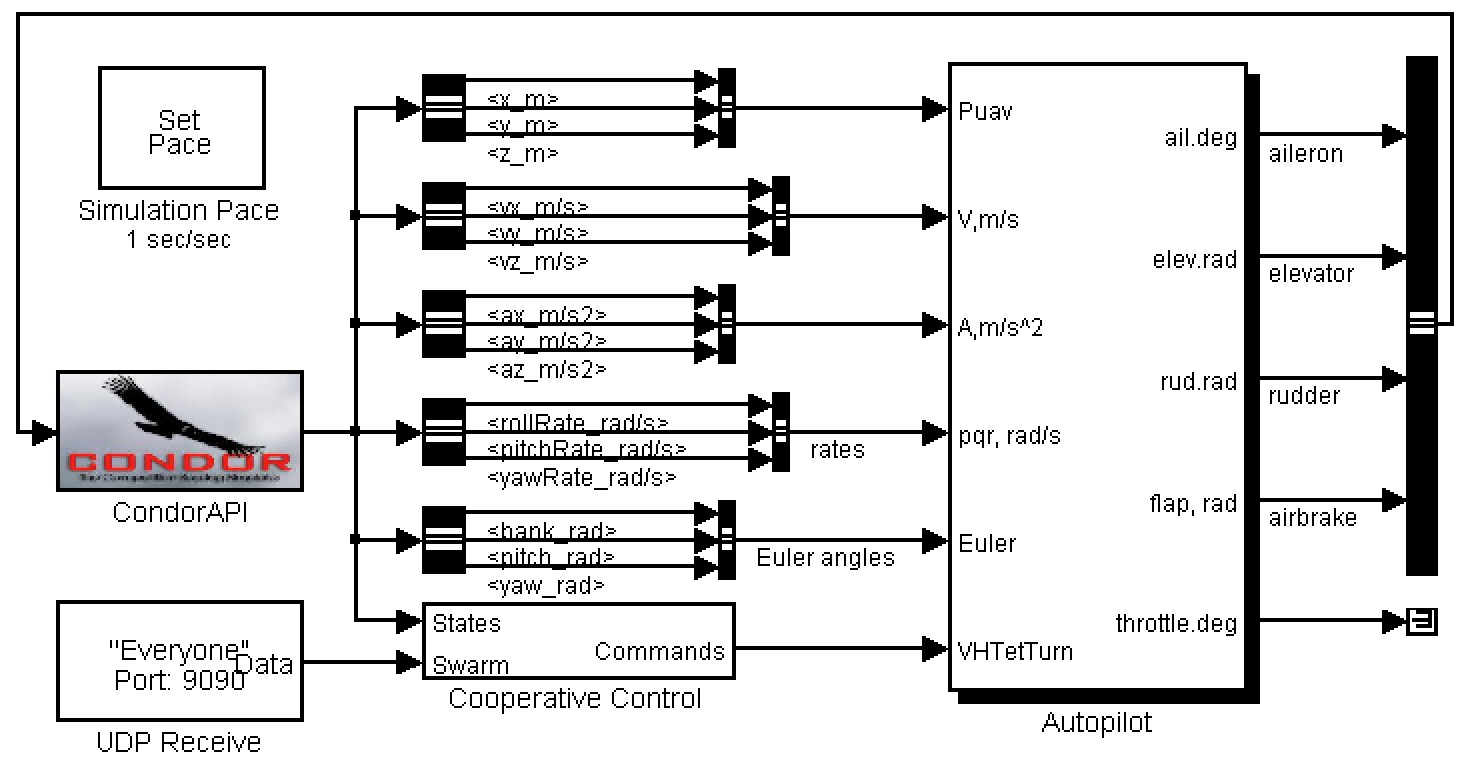
\includegraphics[scale=0.3]{Figures/SIL.eps}
  \caption{Integration of Simulink and Condor capabilities.}
  \label{fig:SIL}
\end{figure}
%%%%%%%%%%
...

\subsection{Potential Capabilities}

...

\section{Principles of Convective Lift Detection and Cooperative Exploitation}
...

\subsection{ Thermals Detection and Exploitation by Single Glider}

Sink polar

Total Energy approach

Guidance of a single glider

\subsection{ Cooperative Strategies}

....

\section{Experimental Results}

Present results of 3 gliders searching for a single thermal in a bounded box. 
One of them finds the thermal, estimates its position and shares knowledge 
with the rest of the team. The other 2 gliders come to the same spot and 
start climbing.

As an illustration of the achieved capabilities, 
Figure.\ref{fig:CoopFlightPaths} represents the cooperative flight of three 
gliders in a simplified scenario introduced above. The gliders start their 
flight simultaneously at the same altitude, and initially spend some time in 
search for thermals. When glider $\#1$ detects an updraft utilizing either of 
the thermal detection approaches, and shares the information about the 
thermal, the other two gliders arrive to the same thermal and successfully 
gain height all together. Time history of the altitude of three cooperative 
gliders is presented next in Figure.\ref{fig:CoopFlightHeight}. The result 
clearly demonstrates the benefits and significant potential of collaborative 
strategies in harvesting the convective updraft energy from the environment.
%%%%%%%%%%
\begin{figure}[thpb]
  \centering
  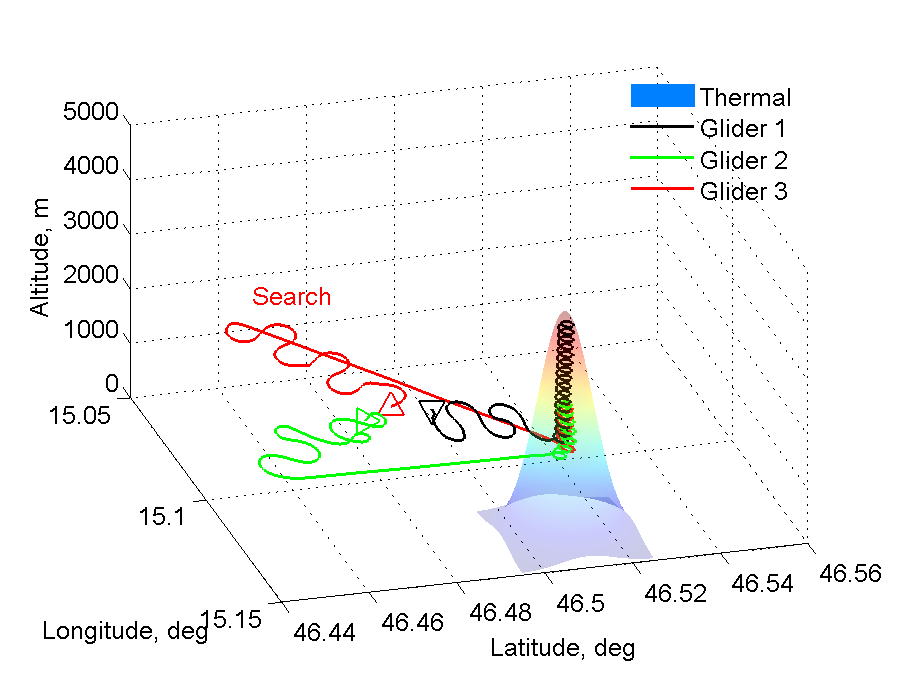
\includegraphics[scale=0.41]{Figures/paths_cooperative_flight.eps}
  \caption{Cooperative flight of three gliders; starting at different locations
  they all converge to the same updraft when glider $\#1$ finds it and
  shares its estimated location.}
  \label{fig:CoopFlightPaths}
\end{figure}
%%%%%%%%%%
%%%%%%%%%%
\begin{figure}[thpb]
  \centering
  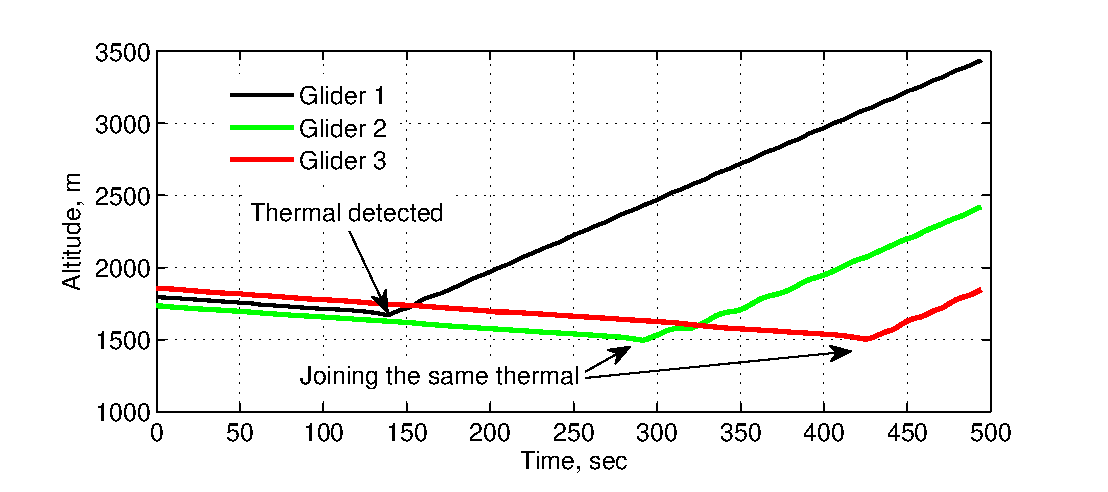
\includegraphics[scale=0.39]{Figures/Coop_gain_altitude.eps}
  \caption{An example of cooperative flight of three gliders.}
  \label{fig:CoopFlightHeight}
\end{figure}

%%%%%%%%%%%%%%%%%%%%%%%%%%%%%%%%%%%%%%%%%%%%%%%%%%%%%%%%%%%%%%%%%%%%%%%%%%%%%%%%
\section*{APPENDIX}

Appendixes can be used to show the snippets of configuration files.

\section*{ACKNOWLEDGMENT}
The project has been supported over the last 3 years by a number of sponsors 
including the NPS Consortium for Robotics and Unmanned Systems Education and 
Research, the Army Research Lab, and "The Multidisciplinary Studies Support 
for USMC Expeditionary Energy Office" program. The authors would like to 
mention the contribution of graduate students Andrew Streenan and Joshua 
Weiss for providing results of their final project and contributing to the 
extensive simulation research.

%%%%%%%%%%%%%%%%%%%%%%%%%%%%%%%%%%%%%%%%%%%%%%%%%%%%%%%%%%%%%%%%%%%%%%%%%%%%%%%%

\bibliographystyle{IEEEtran}
\bibliography{IEEEabrv,iros}



\end{document}
